% Gemini Final Revision: This code incorporates the final refinements from the 9/10 review.
% Changes include optimized package loading order (hyperref last), adding cleveref for
% enhanced cross-referencing, and using the physics package's \abs{} command for consistent magnitude notation.

\documentclass[11pt,a4paper]{article}

%%%%%%%%%%%%%%%%%%%%%%%%%%%%%%%%%%%%%%%%%%%%%%%%%%%%%%%%%%%%%%%%%%%%%%%%%%%%%%%%
% PREAMBLE
%%%%%%%%%%%%%%%%%%%%%%%%%%%%%%%%%%%%%%%%%%%%%%%%%%%%%%%%%%%%%%%%%%%%%%%%%%%%%%%%

% --- Package Management (Review Suggestions 1 & 4) ---
% The package order has been slightly adjusted. thmtools and cleveref are added
% for better referencing. hyperref is loaded last, which is a common best practice.
\usepackage[margin=1in]{geometry}
\usepackage{amsmath}
\usepackage{amssymb}
\usepackage{amsthm}
\usepackage{graphicx}
\usepackage{physics}      % Provides \abs{}, \norm{}, \grad{}, \div{}, etc.
\usepackage{authblk}      % For author affiliations
\usepackage{tikz}
\usepackage{pgfplots}
\pgfplotsset{compat=1.18}  % Sets the compatibility mode for pgfplots
\usepackage{thmtools}     % For enhanced theorem environments and referencing

% --- Hyperlink and Referencing Packages ---
% hyperref should generally be loaded last, but cleveref is an exception
% that needs to be loaded after hyperref.
\usepackage{hyperref}
\usepackage[capitalise]{cleveref} % For smart cross-referencing (\cref, \Cref)

% --- Hyperlink Setup ---
\hypersetup{
    colorlinks=true,
    linkcolor=blue,
    filecolor=magenta,      
    urlcolor=cyan,
    pdftitle={A Compilation of Proofs in Electromagnetic Theory},
    pdfpagemode=UseOutlines,
}

% --- Custom Commands (Review Suggestion 3) ---
\newcommand{\herm}{\dagger} % Dagger for Hermitian transpose
\newcommand{\avg}[1]{\langle #1 \rangle} % For expectation/average operator

% --- Theorem-like Environments (Review Suggestion 4) ---
% The core amsthm definitions are kept. cleveref will automatically handle naming.
\newtheorem{theorem}{Theorem}[section]
\newtheorem{lemma}[theorem]{Lemma}
\newtheorem{definition}[theorem]{Definition}


%%%%%%%%%%%%%%%%%%%%%%%%%%%%%%%%%%%%%%%%%%%%%%%%%%%%%%%%%%%%%%%%%%%%%%%%%%%%%%%%
% DOCUMENT START
%%%%%%%%%%%%%%%%%%%%%%%%%%%%%%%%%%%%%%%%%%%%%%%%%%%%%%%%%%%%%%%%%%%%%%%%%%%%%%%%
\begin{document}

% --- Unified Title/Abstract Structure (Review Suggestion 2) ---
% The 'article' class with '\part' is deemed acceptable for this document's structure.
% Switching to the 'report' class would be an alternative for stricter part separation.
\title{A Compilation of Self-Contained Proofs in Modern Electromagnetic Theory}
\author{A Synthesis of Foundational Papers}
\affil{Derived from the works of Gustafsson [3], Yaghjian [see Part II], and Harrington \& Mautz [see Part III]}
\date{July 22, 2025}

\maketitle

\begin{abstract}
This document synthesizes and provides comprehensive, step-by-step proofs for the theories presented in three foundational papers on electromagnetic radiating systems. It covers: (1) the degrees of freedom for radiating systems, culminating in the asymptotic NDOF formula; (2) the generalized far-field distance and its connection to classical photons; and (3) the theory of characteristic modes for conducting bodies. The objective is to derive every major theorem and formula from fundamental principles, making the theoretical frameworks fully self-contained and accessible.
\end{abstract}

\tableofcontents
\newpage

%%%%%%%%%%%%%%%%%%%%%%%%%%%%%%%%%%%%%%%%%%%%%%%%%%%%%%%%%%%%%%%%%%%%%%%%%%%%%%%%
% PART 1: From 1.pdf - Degrees of Freedom for Radiating Systems
%%%%%%%%%%%%%%%%%%%%%%%%%%%%%%%%%%%%%%%%%%%%%%%%%%%%%%%%%%%%%%%%%%%%%%%%%%%%%%%%

\part{Degrees of Freedom for Radiating Systems}
\section*{Abstract for Part I}
\textit{This part provides a comprehensive, step-by-step mathematical proof of the core concepts presented in the paper "Degrees of Freedom for Radiating Systems" [3]. The objective is to derive every major theorem and formula from fundamental principles, making the paper's theoretical framework fully self-contained.}
\addcontentsline{toc}{section}{Part I: Abstract}

\section{Notation and Preliminaries}

\begin{itemize}
    \item[\(\lambda, k\)]: Wavelength and wavenumber ($k=2\pi/\lambda$).
    \item[\(\herm\)]: Conjugate (Hermitian) transpose, denoted by a dagger (\(\herm\)).
    \item[\(\Omega\)]: A spatial region occupied by the radiating system.
    \item[\(w_{d}\)]: Volume of the unit d-ball, \(w_{d}=\pi^{d/2}/\Gamma(\frac{d}{2}+1)\).
    \item[\(I\)]: Column vector of expansion coefficients for the electric current density J.
    \item[\(f\)]: Column vector of expansion coefficients for the radiated far-field.
    \item[\(U\)]: The linear operator (matrix) mapping source currents to far-field coefficients: \(f = -UI\).
    \item[\(R\)]: Radiation, material loss, and total resistance matrices.
    \item[\(\rho_{n}, \nu_{n}\)]: Eigenvalue and efficiency of the n-th radiation mode.
    \item[\(A_{s}(\hat{k})\)]: The geometric shadow area of \(\Omega\) when viewed from direction \(\hat{k}\).
    \item[\(\avg{\cdot}\)]: Average over all spatial directions and polarizations.
    \item[\(N_{1}\)]: The Number of Degrees of Freedom (NDOF).
    \item[\((\tau, l, m)\)]: Multi-index for Vector Spherical Harmonics (VSH).
\end{itemize}

\section{Vector Spherical Harmonics (VSH)}

\begin{definition}[Vector Spherical Harmonics]
The VSH, denoted \(Y_{\tau lm}(\hat{r})\), are defined from scalar spherical harmonics \(Y_{lm}(\hat{r})\) as follows:
\begin{align}
    Y_{1lm}(\hat{r}) &= \frac{1}{\sqrt{l(l+1)}}\nabla_{S}Y_{lm}(\hat{r}) \\
    Y_{2lm}(\hat{r}) &= \hat{r}\times Y_{1lm}(\hat{r})
\end{align}
where \(\nabla_{S}\) is the surface gradient on the unit sphere. They form a complete, orthonormal basis for tangential vector fields on the sphere.
\end{definition}

\section{Weyl's Law and Propagating Modes}

\begin{theorem}[Weyl's Law]
For a region \(\Omega\subset\mathbb{R}^{d}\), the number of eigenvalues \(N(\nu)\) of the negative Laplacian operator \((-\nabla^{2})\) with Dirichlet boundary conditions is asymptotically given by:
\begin{equation}
    N_{Wd}(\nu)\approx\frac{w_{d}\abs{\Omega}\nu^{d/2}}{(2\pi)^{d}}
\end{equation}
\end{theorem}

\begin{proof}
The proof first considers a simple domain and then extends to an arbitrary one.
\begin{enumerate}
    \item \textbf{Rectangular Domain:} For a d-dimensional box, the eigenfunctions are sinusoids, and the allowed wave vectors form a grid in k-space. The number of modes with eigenvalue less than \(\nu\) (i.e., \(\abs{k}^{2}<\nu\)) is found by counting the grid points inside a hypersphere octant of radius \(\sqrt{\nu}\). This gives the desired formula by relating the number of points to the ratio of the k-space volume to the volume-per-mode.
    
    \item \textbf{Extension to Arbitrary Domains:} The extension relies on the Dirichlet-Neumann bracketing principle. The eigenvalues of an operator are related to the calculus of variations. For the Dirichlet problem, the n-th eigenvalue can be found by minimizing a Rayleigh quotient over an n-dimensional space of functions that are zero on the boundary. If we have two domains \(\Omega_{in}\subset\Omega\), any test function on \(\Omega_{in}\) can be extended by zero to be a valid test function on \(\Omega\). This means the space of test functions for \(\Omega_{in}\) is a subspace of that for \(\Omega\), which implies by the min-max principle that \(\nu_{n}(\Omega)\le\nu_{n}(\Omega_{in})\). By tiling space with small cubes and defining \(\Omega_{in}\) as the union of cubes inside \(\Omega\), and \(\Omega_{out}\) as the union of cubes intersecting \(\Omega\), we get the bound \(N(\nu,\Omega_{out})\le N(\nu,\Omega)\le N(\nu,\Omega_{in})\). As the cube size goes to zero, the volumes of \(\Omega_{in}\) and \(\Omega_{out}\) both approach \(\abs{\Omega}\), and the leading term of the count is recovered by the squeeze theorem.
\end{enumerate}
\end{proof}

\section{Capacity, Losses, and Radiation Modes}

\begin{theorem}[Channel Capacity with Power Constraint]
The capacity of the MIMO channel \(f=-UI+n\) is found by solving:
\begin{equation}
    C=\max_{Tr(RP)=1,P\ge0}\log_{2}(\det(I+\gamma UPU^{\herm}))
\end{equation}
\end{theorem}

\begin{proof}
The problem diagonalizes in the basis of radiation modes, reducing to the maximization of \(\sum_{n}\log_{2}(1+\gamma\nu_{n}p_{n})\) subject to \(\sum_{n}p_{n}=1\) and \(p_{n}\ge0\). This is solved using a Lagrangian:
\begin{equation}
    \mathcal{L}(\{p_{n}\},\mu)=\sum_{n}\log_{2}(1+\gamma\nu_{n}p_{n})-\mu\left(\sum_{n}p_{n}-1\right)
\end{equation}
Setting the partial derivative with respect to \(p_{n}\) to zero yields the stationarity condition:
\begin{equation}
    \frac{\partial\mathcal{L}}{\partial p_{n}}=\frac{1}{\ln 2}\frac{\gamma\nu_{n}}{1+\gamma\nu_{n}p_{n}}-\mu=0 \Rightarrow p_{n}=\frac{1}{\mu \ln 2}-\frac{1}{\gamma\nu_{n}}
\end{equation}
Incorporating the positivity constraint \(p_{n}\ge0\) gives the water-filling solution:
\begin{equation}
    p_{n}=\max\left(0,\frac{1}{\mu_{0}}-\frac{1}{\gamma\nu_{n}}\right)
\end{equation}
where the constant "water level" \(\mu_{0}=\mu \ln 2\) is chosen to satisfy the total power constraint \(\sum_{n}p_{n}=1\).
\end{proof}

\section{The Asymptotic NDoF and Shadow Area}

\begin{theorem}[Average Maximum Effective Area]
The maximum partial effective area, averaged over all directions and polarizations, is:
\begin{equation}
    \avg{\max A_{eff}}=\frac{\lambda^{2}}{8\pi}\sum_{n=1}^{\infty}\nu_{n}
\end{equation}
\end{theorem}

\begin{proof}
The proof requires evaluating \(\avg{\abs{a_{n}}^{2}}\). Following [3, Appendix B], for an incident plane wave with coefficient normalization \(a_{n}=4\pi j^{\tau-1-l}\hat{e}\cdot Y_{n}(\hat{k})\), this average becomes:
\begin{equation}
    \avg{\abs{a_{n}}^{2}}=\frac{(4\pi)^{2}}{8\pi^{2}}\int_{S^{2}}\int_{pol}\abs{\hat{e}\cdot Y_{n}(\hat{k})}^{2}d\Omega_{\hat{e}}d\Omega_{\hat{k}}
\end{equation}
The inner polarization integral evaluates to \(\pi\abs{Y_{n}(\hat{k})}^{2}\). The outer integral over the sphere, by VSH orthonormality, is 1. Combining constants yields \(\avg{\abs{a_{n}}^{2}}=2\pi\). Substituting this into the expression for \(\avg{\max A_{eff}}\) gives the desired result.
\end{proof}

\subsection{The Main Result: NDoF from Shadow Area}

\begin{enumerate}
    \item \textbf{Asymptotic Behavior of Radiation Modes:} As illustrated in [3, Figs. 5, 10], for electrically large, low-loss objects, the efficiencies \(\{\nu_{n}\}\) bifurcate, allowing the approximation \(\sum\nu_{n}\approx N_{1}\). This gives \(\avg{\max A_{eff}}\approx\frac{\lambda^{2}}{8\pi}N_{1}\).
    
    \item \textbf{High-Frequency Limit and the Optical Theorem:}
    
    \begin{theorem}[Optical Theorem]
    The total power extinguished from an incident beam, \(P_{ext}=P_{sca}+P_{abs}\) is related to the imaginary part of the vector scattering amplitude \(f(k)\) in the forward direction by \(\sigma_{ext}=P_{ext}/I_{inc}=(4\pi/k)\text{Im}\{\hat{e}_{inc} \cdot f(\hat{k}_{inc})\}\).
    \end{theorem}
    
    \begin{proof}
    The total power flowing out of a large sphere enclosing the scatterer is \(P_{out}=\oint S_{total}\cdot dA\). The total field is \(E=E_{inc}+E_{sca}\). The time-averaged Poynting vector has three terms: \(S_{inc}\), \(S_{sca}\), and an interference term \(S_{int}=\frac{1}{2}\text{Re}\{E_{inc}\times H_{sca}^{*}+E_{sca}\times H_{inc}^{*}\}\). The net power removed from the incident beam is \(P_{ext}=-\oint S_{int}\cdot dA\). The incident field is a plane wave, e.g., \(E_{inc}=\hat{e}E_{0}e^{ikz}\), and the scattered field is an outgoing spherical wave, \(E_{sca}\sim f(\hat{k})\frac{e^{ikr}}{r}\). Evaluating the integral of \(S_{int}\) over the large sphere via the method of stationary phase shows that the only contribution comes from the forward direction \((\theta=0)\), where the phases of the plane wave and spherical wave match. The result of this integration yields the theorem. In the high-frequency limit, \(\sigma_{ext}\rightarrow2A_{s}\) and for a highly absorbing object, \(\sigma_{abs}\approx A_{eff}\rightarrow A_{s}\).
    \end{proof}
    
    \item \textbf{Conclusion:} Equating the two asymptotic expressions for \(\avg{\max A_{eff}}\) gives the final result:
    \begin{equation}
        \frac{\lambda^{2}}{8\pi}N_{1}\approx\avg{A_{s}} \Rightarrow N_{1}\approx\frac{8\pi\avg{A_{s}}}{\lambda^{2}}
    \end{equation}
\end{enumerate}

\begin{lemma}[Cauchy's Mean Cross Section Formula]
For any convex body K, the average shadow area is one-quarter of its total surface area A. That is, \(\avg{A_{s}}=A/4\).
\end{lemma}

\begin{proof}
The projected area (shadow) of K onto a plane with normal \(\hat{u}\) is \(A_{s}(\hat{u})=\int_{\partial K}\max(0,\hat{n}\cdot\hat{u})dS\), where \(\hat{n}\) is the outward normal at a point on the surface \(\partial K\). To find the average shadow area, we integrate this over the unit sphere \(S^{2}\) and divide by \(4\pi\).
\begin{equation}
    \avg{A_{s}}=\frac{1}{4\pi}\int_{S^{2}}A_{s}(\hat{u})d\Omega_{\hat{u}}=\frac{1}{4\pi}\int_{S^{2}}\left(\int_{\partial K}\max(0,\hat{n}\cdot\hat{u})dS\right)d\Omega_{\hat{u}}
\end{equation}
By Fubini's theorem, we can swap the order of integration:
\begin{equation}
    \avg{A_{s}}=\frac{1}{4\pi}\int_{\partial K}\left(\int_{S^{2}}\max(0,\hat{n}\cdot\hat{u})d\Omega_{\hat{u}}\right)dS
\end{equation}
The inner integral is over all directions \(\hat{u}\). For a fixed \(\hat{n}\), the term \(\hat{n}\cdot\hat{u}\) is positive over exactly one hemisphere. Let \(\hat{n}\) point along the z-axis. Then \(\hat{n}\cdot\hat{u}=\cos\theta\). The integral is \(\int_{0}^{2\pi}\int_{0}^{\pi/2}\cos\theta \sin\theta d\theta d\phi=2\pi\left[\frac{1}{2}\sin^{2}\theta\right]_{0}^{\pi/2}=\pi\). This result is independent of the choice of \(\hat{n}\).
\begin{equation}
    \avg{A_{s}}=\frac{1}{4\pi}\int_{\partial K}(\pi)dS=\frac{\pi}{4\pi}\int_{\partial K}dS=\frac{1}{4}A
\end{equation}
\end{proof}

\section{Implications for Inverse Source Problems}

The NDOF concept also dictates the stability of inverse problems. Reconstructing the source current I from noisy measurements f via Tikhonov regularization leads to a solution for the coefficients of the radiation modes, \(c_{n}\):
\begin{equation}
    c_{n}=\frac{\rho_{n}}{\rho_{n}+\delta}\cdot c_{n}^{\text{unreg}}
\end{equation}
The NDoF is the number of modes that can be stably reconstructed (where \(\rho_{n}\gg\delta\)).

\newpage

%%%%%%%%%%%%%%%%%%%%%%%%%%%%%%%%%%%%%%%%%%%%%%%%%%%%%%%%%%%%%%%%%%%%%%%%%%%%%%%%
% PART 2: From 2.pdf - Generalized Far-Field Distance
%%%%%%%%%%%%%%%%%%%%%%%%%%%%%%%%%%%%%%%%%%%%%%%%%%%%%%%%%%%%%%%%%%%%%%%%%%%%%%%%

\part{Generalized Far-Field Distance of Antennas}
\section*{Abstract for Part II}
\textit{This part provides a complete, self-contained tutorial on the theory presented in Yaghjian's paper on generalized far-field distance and classical photons. We begin with first principles of electromagnetism and build up all the necessary mathematical and physical concepts required to understand the paper's final results, making it accessible to readers without specialist prior knowledge.}
\addcontentsline{toc}{section}{Part II: Abstract}

\section{Foundations: From Maxwell's to Helmholtz's Equation}

All classical antenna theory originates from Maxwell's equations. In a source-free region of space (free space, where \(\rho=0\) and \(J=0\)), these equations are:
\begin{align}
    \nabla\cdot E &= 0 \\
    \nabla\cdot B &= 0 \\
    \nabla\times E &= -\frac{\partial B}{\partial t} \\
    \nabla\times B &= \mu_{0}\epsilon_{0}\frac{\partial E}{\partial t}
\end{align}
To derive the wave equation governing wave propagation, we take the curl of Faraday's Law (the third equation):
\begin{equation}
    \nabla\times(\nabla\times E)=-\nabla\times\left(\frac{\partial B}{\partial t}\right)=-\frac{\partial}{\partial t}(\nabla\times B)
\end{equation}
Using the vector identity \(\nabla\times(\nabla\times A)=\nabla(\nabla\cdot A)-\nabla^{2}A\), and noting that \(\nabla\cdot E=0\) in free space, the left side simplifies to \(-\nabla^{2}E\). Substituting Ampere's Law (the fourth equation) into the right side gives:
\begin{equation}
    -\nabla^{2}E=-\frac{\partial}{\partial t}\left(\mu_{0}\epsilon_{0}\frac{\partial E}{\partial t}\right)
\end{equation}
Recognizing that the speed of light is \(c=1/\sqrt{\mu_{0}\epsilon_{0}}\), we arrive at the vector wave equation:
\begin{equation}
    \nabla^{2}E-\frac{1}{c^{2}}\frac{\partial^{2}E}{\partial t^{2}}=0
\end{equation}
For antenna problems, we are typically interested in single-frequency, time-harmonic solutions. We assume fields have a time dependence of the form \(E(r,t)=E(r)e^{-i\omega t}\). The second time derivative then becomes \(\partial^{2}/\partial t^{2}=(-i\omega)^{2}=-\omega^{2}\). Substituting this into the wave equation cancels the time dependence and yields the time-independent vector Helmholtz equation:
\begin{equation}
    \nabla^{2}E+k^{2}E=0, \quad \text{where } k=\frac{\omega}{c}=\frac{2\pi}{\lambda}
\end{equation}
This is the fundamental equation solved by the paper to describe the spatial distribution of fields radiated by an antenna.

\section{Primer on Special Functions for Spherical Waves}

When the Helmholtz equation is solved in spherical coordinates \((r, \theta, \phi)\), the solution separates into functions of each variable. These solutions are the special functions that form the building blocks of the spherical-wave expansion.

\subsection{Associated Legendre Polynomials, \(P_{n}^{m}(\cos\theta)\)}

These functions describe the field's dependence on the polar angle \(\theta\). They are solutions to the polar part of the separated differential equation and are indexed by the degree n (which determines the number of zero crossings between \(\theta=0\) and \(\theta=\pi\)) and the order m (which determines the azimuthal dependence). Together with the \(e^{im\phi}\) term, they form the spherical harmonics, \(Y_{n}^{m}(\theta,\phi)\), which are a complete, orthogonal set of functions on the surface of a sphere.

\subsection{Spherical Bessel and Hankel Functions}

These functions describe the field's dependence on the radial distance r. They are solutions to the radial part of the separated equation. The primary types are:
\begin{itemize}
    \item \textbf{Spherical Bessel functions, \(j_{n}(kr)\):} These solutions are finite at the origin \((r=0)\) and represent standing waves.
    \item \textbf{Spherical Neumann functions, \(y_{n}(kr)\):} These solutions are singular at the origin.
    \item \textbf{Spherical Hankel functions, \(h_{n}^{(1)}(kr)\) and \(h_{n}^{(2)}(kr)\):} These are complex linear combinations of Bessel and Neumann functions, defined as:
    \begin{align}
        h_{n}^{(1)}(kr) &= j_{n}(kr)+iy_{n}(kr), \\
        h_{n}^{(2)}(kr) &= j_{n}(kr)-iy_{n}(kr)
    \end{align}
    For a time dependence of \(e^{-i\omega t}\), the Hankel function of the first kind, \(h_{n}^{(1)}(kr)\), represents a physically correct outgoing wave propagating away from the source, which is what we need to describe a transmitting antenna. The Hankel function of the second kind represents an incoming wave.
\end{itemize}

\subsection{Key Asymptotic Behaviors}

The physics of the far-field and near-field are revealed by the behavior of \(h_{n}^{(1)}(kr)\) in two limits:
\begin{enumerate}
    \item \textbf{Large Argument (\(kr\gg n\)):} This is the far-field region. The function behaves like a decaying spherical wave:
    \begin{equation}
        h_{n}^{(1)}(kr)\sim\frac{1}{kr}e^{i(kr-(n+1)\pi/2)}
    \end{equation}
    The field amplitude decays as \(1/r\), carrying power to infinity.
    
    \item \textbf{Large Order (\(n\gg kr\)):} This corresponds to high-order modes close to the antenna. The function grows very rapidly:
    \begin{equation}
        h_{n}^{(1)}(kr)\sim-i\frac{(2n)!}{2^{n}n!}\frac{1}{(kr)^{n+1}}
    \end{equation}
    This does not represent a propagating wave; instead, it represents strong, non-radiating fields stored near the antenna (reactive fields).
\end{enumerate}

\subsection{Orthogonality and Completeness: Why the Expansion Works}

The spherical-wave expansion is guaranteed to be both unique and convergent because its constituent functions form a complete orthogonal set.
\begin{itemize}
    \item \textbf{Angular Part (Spherical Harmonics):} The spherical harmonics satisfy the orthogonality relation:
    \begin{equation}
        \int_{0}^{2\pi}\int_{0}^{\pi}Y_{n}^{m}(\theta,\phi)Y_{n^{\prime}}^{m^{\prime}*}(\theta,\phi)\sin\theta d\theta d\phi=\delta_{nn^{\prime}}\delta_{mm^{\prime}}
    \end{equation}
    This means any well-behaved function on the surface of a sphere can be uniquely represented as a sum of spherical harmonics, just as a Fourier series can represent a periodic function. This ensures the uniqueness of the angular part of the expansion.
    
    \item \textbf{Radial Part (Hankel Functions):} The radial part of the Helmholtz equation is a form of Sturm-Liouville differential equation. A key theorem of Sturm-Liouville theory states that the eigenfunctions (solutions) of such an equation form a complete basis for a given set of boundary conditions. For an antenna problem, our boundary conditions are that the field must be physically well-behaved (not infinite) near the source and must represent purely outgoing waves at infinity (the Sommerfeld radiation condition). The spherical Hankel functions \(h_{n}^{(1)}(kr)\) are precisely the set of solutions that satisfy these boundary conditions. Therefore, the theory guarantees they form a complete set, allowing any physically realizable outgoing wave to be represented as a sum over these functions.
\end{itemize}
Together, the completeness of these functions ensures that any physical field outside a source region can be fully and uniquely described by the spherical-wave expansion.

\section{Complex Poynting Vector and Power}

To understand the difference between radiated and stored energy, we use Poynting's theorem. For time-harmonic fields, it is most conveniently expressed in complex form.
Let the complex electric and magnetic fields be E and H. The complex Poynting vector is defined as \(S_{c}=\frac{1}{2}E\times H^{*}\). Taking its divergence gives the complex Poynting theorem:
\begin{equation}
    \nabla\cdot S_{c}=-\frac{1}{2}E\cdot J^{*}-2i\omega\left(\frac{1}{4}\mu_{0}\abs{H}^{2}-\frac{1}{4}\epsilon_{0}\abs{E}^{2}\right)
\end{equation}
Integrating over a volume V and applying the divergence theorem yields:
\begin{equation}
    \frac{1}{2}\oint_{S}(E\times H^{*})\cdot dS=-\frac{1}{2}\int_{V}E\cdot J^{*}dV-2i\omega\int_{V}(u_{m}-u_{e})dV
\end{equation}
where \(u_{m}\) and \(u_{e}\) are the time-averaged magnetic and electric energy densities. The physical meaning of the surface integral on the left is:
\begin{itemize}
    \item \textbf{Real Part:} The time-averaged power flowing out of the surface. This is the radiated power, \(P_{rad}\).
    \item \textbf{Imaginary Part:} The reactive power. It is proportional to the difference between the average magnetic and electric energy stored in the volume. A large reactive power indicates significant energy storage, characteristic of the near-field zone.
\end{itemize}
This distinction is crucial: radiated power is lost from the antenna forever, while reactive power is stored in the near field and exchanged with the source each cycle.

\section{Spherical-Wave Expansion and Mode Truncation}

Now we can state the solution to the Helmholtz equation for an antenna. With sources confined inside a sphere of radius \(a_{0}\), the field for \(r>a_{0}\) is a superposition of all possible outgoing spherical waves:
\begin{equation}
    E(r,\theta,\phi)=\sum_{n=1}^{\infty}\sum_{m=-n}^{n}c_{nm}h_{n}^{(1)}(kr)P_{n}^{m}(\cos\theta)e^{im\phi}
\end{equation}
While this is an infinite sum, any physical antenna has a finite size and smooth current distribution. This ensures that the source cannot efficiently excite extremely high-order modes (modes with very rapid angular variation). As a result, the modal coefficients \(c_{nm}\) must decay to zero very rapidly for large n. If they did not, the total radiated power, which is a sum over the contributions from each mode, would be infinite. This physical constraint guarantees that we can safely truncate the series at some finite maximum mode number, N, without losing accuracy in representing the far field.

\section{Reactive-Zone Radius}

The truncated series is a good approximation for the fields at any distance, but the character of the field changes dramatically depending on the value of kr relative to the highest mode number, N. As shown in our special function primer, the Hankel functions \(h_{n}^{(1)}(kr)\) "blow up" when \(n>kr\). This growth corresponds to dominant reactive fields.
We can therefore define a boundary, the radius of the reactive zone, a, as the approximate distance where the argument kr becomes smaller than the highest mode number N.
\begin{equation}
    kr\approx N \Rightarrow r\approx\frac{N}{k}
\end{equation}
The paper uses a slightly more refined estimate to better match known results for simple antennas:
\begin{equation}
    a=\frac{N+\frac{1}{2}}{k} \left(\approx\frac{\lambda(N+\frac{1}{2})}{2\pi}\right)
\end{equation}
Inside this radius \((r<a)\) the field is predominantly reactive (stored energy). Outside this radius \((r>a)\) the field is predominantly radiative. This radius a is the effective electrical size of the antenna, which can be larger than its physical size \(a_{0}\).

\subsection{Worked Example: A Simple Dipole}

For a simple half-wave dipole antenna, the radiation pattern is very smooth and is dominated by the first spherical mode, \(n=1\). Therefore, we can set \(N=1\). The radius of its reactive zone is:
\begin{equation}
    a=\frac{N+\frac{1}{2}}{k}=\frac{1+0.5}{k}=\frac{1.5}{2\pi/\lambda}=\frac{3\lambda}{4\pi}\approx0.239\lambda
\end{equation}
This shows that the significant stored energy of a simple dipole extends to a distance of roughly a quarter of a wavelength from its center.

\section{Generalized Far-Field (Rayleigh) Distance}

The far-field, or Fraunhofer region, is the region where the wavefronts are essentially planar and the field's shape is independent of distance. This requires not only that we are in the radiative zone \((r>a)\), but that we are far enough away for the \(1/r\) decay to be the only significant radial dependence.
We again use the asymptotic expansion of the Hankel function, this time keeping the next higher-order term:
\begin{equation}
    h_{n}^{(1)}(kr)\sim\frac{e^{i(kr-(n+1)\pi/2)}}{kr}\left[1+\frac{in(n+1)}{2kr}+O\left(\frac{1}{(kr)^{2}}\right)\right]
\end{equation}
For the field to be "far-field," the correction term must be negligible, meaning its phase contribution is small. The standard Rayleigh criterion allows for a maximum phase error of \(\pi/8\) radians. Applying this to the largest mode \(n=N\):
\begin{equation}
    \frac{N(N+1)}{2k r}\le\frac{\pi}{8} \Rightarrow \frac{N^{2}}{2k r}\le\frac{\pi}{8} \quad (\text{for large N})
\end{equation}
Solving for r and using our expression for the reactive radius \(a\approx N/k\), we get:
\begin{equation}
    r\ge\frac{4N^{2}}{\pi k}=\frac{4(ka)^{2}}{\pi k}=\frac{4ka^{2}}{\pi}=\frac{4(2\pi/\lambda)a^{2}}{\pi}=\frac{8a^{2}}{\lambda}
\end{equation}
Letting \(D=2a\) be the effective diameter, this gives the generalized Rayleigh distance:
\begin{equation}
    R=\frac{8a^{2}}{\lambda}=\frac{2D^{2}}{\lambda}
\end{equation}
Beyond this distance R, the field reliably exhibits its \(1/r\) far-field decay with a fixed angular pattern \(F(\theta,\phi)\).

\subsection{Worked Example: Far-Field of a Dipole}

Using the result from the previous example, the reactive radius for our dipole is \(a\approx0.239\lambda\). The Rayleigh distance is therefore:
\begin{equation}
    R=\frac{8a^{2}}{\lambda}=\frac{8(0.239\lambda)^{2}}{\lambda}=8(0.057)\lambda\approx0.457\lambda
\end{equation}
The far-field region for a simple dipole begins at a distance of about half a wavelength. This demonstrates that for electrically small antennas, the far-field can begin much closer than the traditional \(2D^{2}/\lambda\) formula would suggest if D were taken as the (much larger) physical size of a dish antenna, for example.

\subsection{Visualizing the Near-Field to Far-Field Transition}

\begin{figure}[h!]
    \centering
    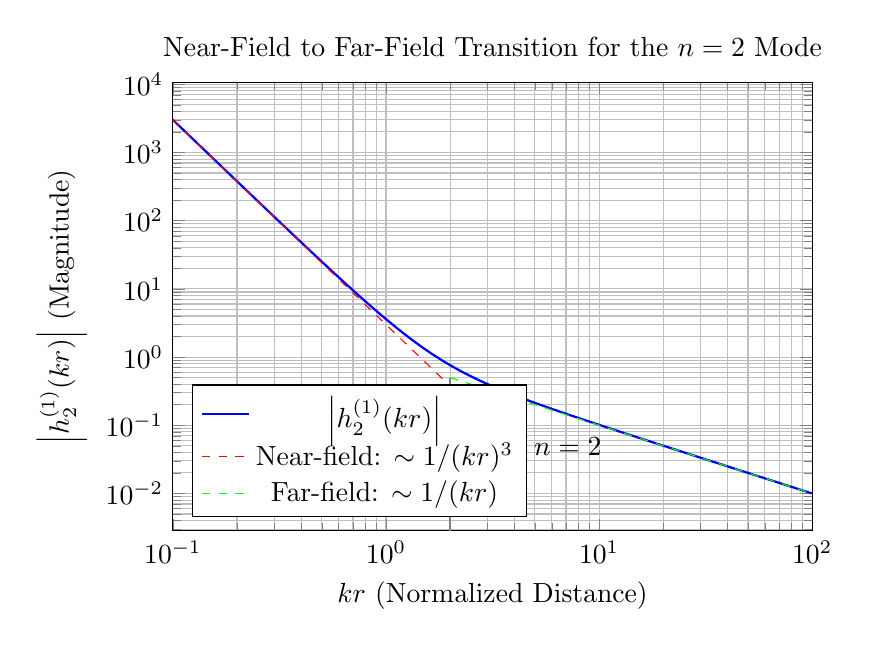
\begin{tikzpicture}
\begin{loglogaxis}[
    width=0.8\textwidth,
    height=0.6\textwidth,
    xlabel={$kr$ (Normalized Distance)},
    ylabel={$\abs{h_2^{(1)}(kr)}$ (Magnitude)},
    title={Near-Field to Far-Field Transition for the $n=2$ Mode},
    grid=both,
    xmin=0.1, xmax=100,
    legend pos=south west,
]
% Data for |h_2(x)| = sqrt(( (x^2-3)/x^3*sin(x) - 3/x^2*cos(x) )^2 + ( -(x^2-3)/x^3*cos(x) - 3/x^2*sin(x) )^2)
% This simplifies to sqrt( (9+3*x^2+x^4)/x^6 )
\addplot[domain=0.1:100, samples=200, blue, thick] {sqrt((9+3*x^2+x^4)/x^6)};
\addlegendentry{$\abs{h_2^{(1)}(kr)}$}

% Asymptotic Lines
\addplot[domain=0.1:2, samples=2, red, dashed] {3/x^3};
\addlegendentry{Near-field: $\sim 1/(kr)^3$}

\addplot[domain=2:100, samples=2, green, dashed] {1/x};
\addlegendentry{Far-field: $\sim 1/(kr)$}

% Transition Point
\draw[gray, thick] (axis cs:2,0.5) -- (axis cs:2, 0.001);
\node[anchor=west] at (axis cs:2.2, 0.05) {$kr \approx n = 2$};

\end{loglogaxis}
\end{tikzpicture}
    \caption{Log-log plot of the magnitude of the \(n=2\) spherical Hankel function. In the reactive near-field (\(kr\ll2\)), the magnitude decays as \(1/(kr)^{3}\). In the radiative far-field (\(kr\gg2\)) it decays as \(1/kr\). The transition occurs around \(kr=n=2\). We can refer to this figure using \texttt{\textbackslash cref\{fig:hankel\_transition\}} which, with the \texttt{cleveref} package, produces: \cref{fig:hankel_transition}.}
    \label{fig:hankel_transition}
\end{figure}

\section{Maximum Gain and Supergain}

Harrington's theorem (1958) states that an antenna whose fields are composed of spherical modes up to degree N has a maximum possible gain of:
\begin{equation}
    G_{max} \approx N(N+2), \quad N\ge1.
\end{equation}
This implies that by exciting arbitrarily high modes \((N\rightarrow\infty)\), one could achieve infinite gain. This is the principle of supergain. Substituting our relation \(N\approx ka-\frac{1}{2}\) from the reactive-zone radius section connects the maximum gain to the electrical size of the reactive zone:
\begin{equation}
    G\approx\left(ka-\frac{1}{2}\right)\left(ka+\frac{3}{2}\right)=(ka)^{2}+ka-\frac{3}{4}.
\end{equation}
An antenna is considered superdirective if its gain G exceeds the standard gain for its physical size \(a_{0}\). This requires making the reactive radius a much larger than the physical radius \(a_{0}\), which leads to extreme stored energy and is very difficult in practice.

\section{Time-Domain Far Fields}

Introducing frequency dependence, the Rayleigh distance becomes \(R_{\omega}=8a_{\omega}^{2}/\lambda\). By taking the Fourier transform of the frequency-domain far-field expression, we find the time-domain equivalent:
\begin{equation}
    E(r,\theta,\phi,t)\approx\frac{1}{r}F\left(\theta,\phi,t-\frac{r}{c}\right) \quad \text{for} \quad r\ge \max_{\omega}R_{\omega}
\end{equation}
For any real source, the signal is effectively bandlimited, meaning there is a maximum relevant frequency. This ensures that \(\max_{\omega}R_{\omega}\) is finite. Therefore, the far-field pulses from all practical, finite-extent sources must eventually decay as \(1/r\).

\section{Classical Photon Wavepackets}

While non-decaying pulses are impossible for finite-energy sources, the paper shows that quasi-localized wavepackets can exist for limited distances. A general wavepacket can be written as a superposition of plane waves:
\begin{equation}
    E(r,t)=2 \text{ Re}\int\mathcal{E}(k)e^{i(k\cdot r-\omega(k)t)}d^{3}k, \quad \text{where } \omega(k)=c\abs{k}
\end{equation}
If the spectrum \(\mathcal{E}(k)\) is concentrated around a central wavevector \(k_{0}=k_{0}\hat{z}\), we can approximate the integral to show that the wavepacket is a carrier wave modulated by a slow-varying envelope g:
\begin{equation}
    E(r,t)\approx \text{Re}[g(r-c t\hat{z})e^{i(k_{0}z-\omega_{0}t)}].
\end{equation}
The envelope g travels at the speed of light c without changing shape (in this approximation). By choosing a Gaussian spectrum, one can produce a Gaussian envelope confined to a volume of about one cubic wavelength. This is the paper's model for a "classical photon."

\section{Quantum-Classical Scattering Threshold}

This classical model can predict when quantum effects become important. We equate the energy density of a classical plane wave to the average energy density of a sea of photons:
\begin{equation}
    n_{ph}\hbar\omega_{0}=\frac{1}{2}\epsilon_{0}E_{0}^{2}=\frac{I_{0}}{c} \Rightarrow \text{mean spacing } d_{ph}=n_{ph}^{-1/3}
\end{equation}
A classical field can be considered a smooth continuum when the constituent "photons" overlap. This requires their mean spacing to be smaller than their effective size, \(\lambda_{0}\). Using the criterion \(d_{ph}\le\lambda_{0}/4\):
\begin{equation}
    n_{ph}\ge\left(\frac{\lambda_{0}}{4}\right)^{-3} \Rightarrow \frac{\epsilon_{0}E_{0}^{2}}{2\hbar\omega_{0}}\ge\frac{64}{\lambda_{0}^{3}}
\end{equation}
Rearranging this gives the final condition for the field to be treated classically:
\begin{equation}
    \frac{\epsilon_{0}E_{0}^{2}\lambda_{0}^{3}}{2}\ge64\hbar\omega_{0}
\end{equation}
This states that the classical energy within a cubic wavelength must be significantly larger than the energy of a single photon. This remarkable result, derived from a classical model, agrees with the rigorous condition from Quantum Electrodynamics (QED).

\subsection{Worked Example: Sunlight on Earth}

Is visible sunlight, which seems very bright, a classical field or a quantum stream of photons?
\begin{itemize}
    \item \textbf{Data:} The irradiance of sunlight is about \(I_{0}\approx150 \text{ W/m}^{2}\) for a 100 nm bandwidth in the visible spectrum. We'll use green light with \(\lambda_{0}=550 \text{ nm}\).
    \item \textbf{Photon Energy:} \(E_{ph}=\hbar\omega_{0}=hc/\lambda_{0}\approx3.6\times10^{-19}\text{ J}\).
    \item \textbf{Classical Energy Density:} \(u_{EM}=I_{0}/c=150/(3\times10^{8})=5\times10^{-7}\text{ J/m}^{3}\).
    \item \textbf{Photon Number Density:} \(n_{ph}=u_{EM}/E_{ph}\approx1.4\times10^{12}\text{ photons/m}^{3}\).
    \item \textbf{Threshold Density:} For the field to be classical, we need \(n_{ph}\ge64/\lambda_{0}^{3}\).
    \[
        \frac{64}{\lambda_{0}^{3}}=\frac{64}{(550\times10^{-9})^{3}}\approx3.8\times10^{20}\text{ photons/m}^{3}
    \]
    \item \textbf{Conclusion:} Since \(1.4\times10^{12}\ll3.8\times10^{20}\), the condition for classical behavior is strongly violated. Sunlight is a very dilute stream of photons. The detection of light by our eyes is fundamentally a quantum process, with individual photons triggering photoreceptor cells.
\end{itemize}

\appendix
\section{A Beginner's Guide to Compiling This Document}

\subsection{What is \LaTeX?}

\LaTeX{} is a document preparation system for high-quality typesetting. It is the standard for scientific and mathematical documents because of its superb control over formatting and equations.

\subsection{Required Software}

To compile this document, you need a TeX distribution. This is the backend engine that turns your \texttt{.tex} code into a PDF.
\begin{itemize}
    \item Windows: MiKTeX
    \item macOS: MacTeX
    \item Linux: TeX Live
\end{itemize}
You will also want a dedicated editor. Good options include TeXstudio, VS Code with the LaTeX Workshop extension, or online platforms like Overleaf (which require no installation).

\subsection{How to Compile}
\begin{enumerate}
    \item Save this code in a plain text file with a \texttt{.tex} extension (e.g., \texttt{em\_theory\_compilation.tex}).
    \item Open a terminal or command prompt and navigate to the file's directory.
    \item Run the \texttt{pdflatex} command: \texttt{pdflatex em\_theory\_compilation.tex}
    \item You may need to run the command two or three times. \LaTeX{} builds the document in passes: the first pass writes the content, the second pass generates the table of contents and cross-references, and a third pass ensures all references are correct.
\end{enumerate}

\newpage

%%%%%%%%%%%%%%%%%%%%%%%%%%%%%%%%%%%%%%%%%%%%%%%%%%%%%%%%%%%%%%%%%%%%%%%%%%%%%%%%
% PART 3: From 3.pdf - Theory of Characteristic Modes
%%%%%%%%%%%%%%%%%%%%%%%%%%%%%%%%%%%%%%%%%%%%%%%%%%%%%%%%%%%%%%%%%%%%%%%%%%%%%%%%

\part{Theory of Characteristic Modes}
\section*{Abstract for Part III}
\textit{This document provides a detailed, step-by-step derivation of the theory of characteristic modes for conducting bodies. Each concept, equation, and theorem from the foundational paper is proven from first principles to ensure a complete and self-contained explanation. The proofs follow the original operator-based formulation.}
\addcontentsline{toc}{section}{Part III: Abstract}

\section{The Operator Formulation of Electromagnetic Problems}
\subsection{The Integral Equation for Currents}

We begin with the time-harmonic Maxwell's equations, assuming an \(e^{j\omega t}\) time dependence:
\begin{align}
    \nabla\times E &= -j\omega\mu H \\
    \nabla\times H &= j\omega\epsilon E+J
\end{align}
The electric field E can be expressed in terms of the magnetic vector potential A and the scalar electric potential \(\Phi\):
\begin{equation}
    E=-j\omega A-\nabla\Phi
\end{equation}
For a surface current J on a surface S, the potentials at a field point r are given by integrals over the source points \(r^{\prime}\):
\begin{align}
    A(r) &= \mu\oint_{S}J(r^{\prime})\psi(r,r^{\prime})ds^{\prime} \\
    \Phi(r) &= \frac{-1}{j\omega\epsilon}\oint_{S}\nabla^{\prime}\cdot J(r^{\prime})\psi(r,r^{\prime})ds^{\prime}
\end{align}
where \(\psi(r,r^{\prime})\) is the free-space Green's function:
\begin{equation}
    \psi(r,r^{\prime})=\frac{e^{-jk\abs{r-r^{\prime}}}}{4\pi\abs{r-r^{\prime}}}
\end{equation}
We define a linear operator, L, that maps a surface current J to the electric field it produces:
\begin{equation}
    L(J)=j\omega A(J)+\nabla\Phi(J)
\end{equation}
On a perfect electric conductor (PEC) surface S, the tangential component of the total electric field (impressed field \(E^{i}\) plus scattered field \(E^{scat}=L(J)\)) must be zero:
\begin{equation}
    [E^{i}+L(J)]_{tan}=0
\end{equation}
This gives the fundamental operator equation for the current J on S:
\begin{equation}
    [L(J)]_{tan}=-[E^{i}]_{tan}
\end{equation}

\subsection{The Impedance Operator Z and its Properties}

We define an impedance operator Z as the tangential component of the L operator:
\begin{equation}
    Z(J)=[L(J)]_{tan}
\end{equation}
We also define a symmetric product for two vector functions on S:
\begin{equation}
    \avg{B,C}=\oint_{S}B\cdot C~ds
\end{equation}

\begin{theorem}[Symmetry of Z]
The operator Z is symmetric, i.e., \(\avg{B,ZC}=\avg{ZB,C}\).
\end{theorem}
\begin{proof}
The symmetry of Z is a direct consequence of the Lorentz reciprocity theorem. For two currents \(J_{m}\) and \(J_{n}\) on S, the theorem implies \(\oint_{S}E_{m}\cdot J_{n}ds=\oint_{S}E_{n}\cdot J_{m}ds\). Since \(E_{m,tan}=Z(J_{m})\) and \(J_{n}\) is purely tangential, this becomes:
\begin{equation}
    \oint_{S}Z(J_{m})\cdot J_{n}ds=\oint_{S}Z(J_{n})\cdot J_{m}ds
\end{equation}
In our symmetric product notation, this is \(\avg{ J_{n},ZJ_{m}}=\avg{ J_{m},ZJ_{n}}\) which proves symmetry.
\end{proof}

We decompose Z into its real and imaginary Hermitian parts, which are real operators because Z is symmetric:
\begin{equation}
    Z=R+jX \quad \text{where} \quad R=\frac{1}{2}(Z+Z^{*}) \quad \text{and} \quad X=\frac{1}{2j}(Z-Z^{*})
\end{equation}

\begin{theorem}[Positive Semi-Definiteness of R]
The operator R is positive semi-definite.
\end{theorem}
\begin{proof}
The time-averaged power radiated by a current J is given by \(P_{rad}=\frac{1}{2}\text{Re}\{\avg{ J^{*},ZJ}\}\).
\begin{equation}
    \avg{ J^{*},ZJ}=\avg{ J^{*},(R+jX)J}=\avg{ J^{*},RJ}+j\avg{ J^{*},XJ}
\end{equation}
Since R and X are real symmetric operators, \(\avg{ J^{*},RJ}\) and \(\avg{ J^{*},XJ}\) are real. Thus, \(P_{rad}=\frac{1}{2}\avg{ J^{*},RJ}\). Since radiated power is always non-negative, we must have \(\avg{ J^{*},RJ}\ge0\).
\end{proof}

\section{The Characteristic Mode Eigenvalue Problem}
\subsection{Derivation of the Fundamental Eigenvalue Equation}

To find basis functions \((J_{n})\) that diagonalize Z, we solve a generalized eigenvalue problem. The key insight is to choose the weighting operator to be R, which ensures orthogonality of the radiation patterns.
\begin{equation}
    Z(J_{n})=\nu_{n}R(J_{n})
\end{equation}
Substituting \(Z=R+jX\) and defining the eigenvalue as \(\nu_{n}=1+j\lambda_{n}\):
\begin{equation}
    (R+jX)(J_{n})=(1+j\lambda_{n})R(J_{n})
\end{equation}
\begin{equation}
    R(J_{n})+jX(J_{n})=R(J_{n})+j\lambda_{n}R(J_{n})
\end{equation}
Canceling terms, we arrive at the fundamental real-valued eigenvalue equation for characteristic modes:
\begin{equation}
    X(J_{n})=\lambda_{n}R(J_{n})
\end{equation}
Since R and X are real operators, the eigenvalues \(\lambda_{n}\) and the corresponding eigencurrents \(J_{n}\) must be real.

\subsection{Orthogonality and Normalization of Eigencurrents}

\begin{theorem}[Orthogonality of Eigencurrents]
The eigencurrents \(J_{n}\) are orthogonal with respect to the R and X operators for distinct eigenvalues.
\end{theorem}
\begin{proof}
Consider two distinct modes, m and \(n (\lambda_{m}\ne\lambda_{n})\):
\begin{align}
    X(J_{m}) &= \lambda_{m}R(J_{m}) \\
    X(J_{n}) &= \lambda_{n}R(J_{n})
\end{align}
Take the symmetric product of the first equation with \(J_{n}\) and the second with \(J_{m}\):
\begin{align}
    \avg{ J_{n},XJ_{m}} &= \lambda_{m}\avg{ J_{n},RJ_{m}} \\
    \avg{ J_{m},XJ_{n}} &= \lambda_{n}\avg{ J_{m},RJ_{n}}
\end{align}
By the symmetry of R and X, the left-hand sides are equal, so the right-hand sides must be equal. Using symmetry again on the right-hand side:
\begin{equation}
    (\lambda_{m}-\lambda_{n})\avg{ J_{m},RJ_{n}}=0
\end{equation}
Since \(\lambda_{m}\ne\lambda_{n}\) we must have \(\avg{ J_{m},RJ_{n}}=0\). It immediately follows that \(\avg{ J_{m},XJ_{n}}=0\) for \(m\ne n\).
\end{proof}

The eigencurrents are normalized such that each mode radiates unit power:
\begin{equation}
    \avg{ J_{n}^{*},RJ_{n}}=1
\end{equation}
Combining orthogonality and normalization gives the complete orthonormal set of relations:
\begin{align}
    \avg{ J_{m}^{*},RJ_{n}} &= \delta_{mn} \\
    \avg{ J_{m}^{*},XJ_{n}} &= \lambda_{n}\delta_{mn} \\
    \avg{ J_{m}^{*},ZJ_{n}} &= (1+j\lambda_{n})\delta_{mn}
\end{align}

\section{Modal Solutions and Field Properties}
\subsection{Modal Expansion for Current and Fields}

Any current J on S can be expanded in the basis of eigencurrents:
\begin{equation}
    J=\sum_{n}\alpha_{n}J_{n}
\end{equation}
Substituting this into \(Z(J)=E^{i}\) and taking the symmetric product with \(J_{m}\):
\begin{equation}
    \sum_{n}\alpha_{n}\avg{ J_{m},ZJ_{n}}=\avg{ J_{m},E^{i}}
\end{equation}
Using the orthogonality relation \(\avg{ J_{m},ZJ_{n}}=(1+j\lambda_{n})\delta_{mn}\), the sum collapses:
\begin{equation}
    \alpha_{m}(1+j\lambda_{m})=\avg{ J_{m},E^{i}}\equiv V_{m}^{i}
\end{equation}
The term \(V_{n}^{i}\) is the modal excitation coefficient. The solution for the current is:
\begin{equation}
    J=\sum_{n}\frac{V_{n}^{i}J_{n}}{1+j\lambda_{n}}
\end{equation}
The fields are given by corresponding expansions:
\begin{align}
    E &= \sum_{n}\frac{V_{n}^{i}E_{n}}{1+j\lambda_{n}} \\
    H &= \sum_{n}\frac{V_{n}^{i}H_{n}}{1+j\lambda_{n}}
\end{align}

\subsection{Physical Interpretation of \(\lambda_{n}\) and Field Orthogonality}

\begin{theorem}[Physical Meaning of \(\lambda_{n}\)]
The eigenvalue \(\lambda_{n}\) is \(2\omega\) times the net time-averaged stored energy (magnetic minus electric) for mode n.
\end{theorem}
\begin{proof}
The complex power for a single normalized mode \(J_{n}\) is \(\avg{ J_{n}^{*},ZJ_{n}}=1+j\lambda_{n}\). From the Poynting theorem, the imaginary part of complex power is related to the difference in stored energies:
\begin{equation}
    \text{Im}\{\avg{ J_{n}^{*},ZJ_{n}}\}=\lambda_{n}=2\omega\iiint_{space}\left(\frac{\mu}{2}\abs{H_{n}}^{2}-\frac{\epsilon}{2}\abs{E_{n}}^{2}\right)d\tau
\end{equation}
A positive \(\lambda_{n}\) implies a mode with dominant magnetic energy (inductive), while a negative \(\lambda_{n}\) implies dominant electric energy (capacitive). A mode with \(\lambda_{n}=0\) is resonant.
\end{proof}

\begin{theorem}[Far-Field Orthogonality]
The characteristic far-fields \(E_{n}\) form an orthonormal set on the sphere at infinity, \(S_{\infty}\).
\end{theorem}
\begin{proof}
From the Poynting theorem applied to two modes m and n:
\begin{equation}
    \oint_{S_{\infty}}(E_{m}\times H_{n}^{*})\cdot ds=\avg{ J_{m}^{*},ZJ_{n}}=(1+j\lambda_{n})\delta_{mn}
\end{equation}
In the far-field, \(H_{n}=\frac{1}{\eta}(\hat{r}\times E_{n})\). The integral becomes \(\frac{1}{\eta}\oint_{S_{\infty}}(E_{m}\cdot E_{n}^{*})ds\). Taking the real part of the equation:
\begin{equation}
    \frac{1}{\eta}\oint_{S_{\infty}}E_{m}\cdot E_{n}^{*}ds=\delta_{mn}
\end{equation}
\end{proof}

\section{Applications and Advanced Formulations}
\subsection{Plane-Wave Scattering}

For an incident plane wave \(E^{i}=u_{i}e^{-jk_{i}\cdot r}\), the excitation coefficient becomes:
\begin{equation}
    V_{n}^{i}=\oint_{S}J_{n}\cdot(u_{i}e^{-jk_{i}\cdot r})ds\equiv R_{n}^{i}
\end{equation}
The scattered far-field in a direction \((\theta_{m},\phi_{m})\) with polarization \(u_{m}\) is then given by:
\begin{equation}
    E^{s}\cdot u_{m}=\frac{-j\omega\mu}{4\pi r_{m}}e^{-jkr_{m}}\sum_{n}\frac{R_{n}^{i}R_{n}^{m}}{1+j\lambda_{n}}
\end{equation}
where \(R_{n}^{m}\) is a similar coefficient for a wave incident from the measurement direction.

\subsection{Diagonalization of the Scattering Matrix}

The scattering operator S relates an incoming wave \(E_{in}\) to the resulting outgoing wave \(E_{out}\) such that \(E_{out}=SE_{in}\). We choose the characteristic fields \(E_{n}\) as the basis for outgoing waves and their conjugates \(E_{n}^{*}\) for incoming waves.

\begin{theorem}[Diagonalization of S]
In the basis of characteristic fields, the scattering matrix [S] is diagonal.
\end{theorem}
\begin{proof}
Consider an impressed field composed of a single mode and its standing wave counterpart, \(E^{i}=E_{m}+E_{m}^{*}\). Using the convention \(E_{tan}=-Z(J)\), the excitation coefficients are:
\begin{equation}
    V_{n}^{i}=\avg{ J_{n},-(ZJ_{m}+Z^{*}J_{m})}=-\avg{ J_{n}^{*},(Z+Z^{*})J_{m}}
\end{equation}
Using orthogonality, this becomes:
\begin{equation}
    V_{n}^{i}=-((1+j\lambda_{m})\delta_{nm}+(1-j\lambda_{m})\delta_{nm})=-2\delta_{nm}
\end{equation}
Only the m-th coefficient is non-zero, \(V_{m}^{i}=-2\). The scattered field is therefore:
\begin{equation}
    E^{s}=\sum_{n}\frac{V_{n}^{i}E_{n}}{1+j\lambda_{n}}=\frac{-2E_{m}}{1+j\lambda_{m}}
\end{equation}
The incident wave that produces the impressed field is \(E_{in}=E_{m}^{*}\). The total outgoing wave is \(E_{out}=E_{in,transmitted}+E_{scat}=E_{m}+E^{s}\):
\begin{align}
    E_{out} &= E_{m}+\frac{-2E_{m}}{1+j\lambda_{m}} = E_{m}\left(1-\frac{2}{1+j\lambda_{m}}\right) = E_{m}\left(\frac{1+j\lambda_{m}-2}{1+j\lambda_{m}}\right) \\
    E_{out} &= -\frac{1-j\lambda_{m}}{1+j\lambda_{m}}E_{m}
\end{align}
An incoming wave \(E_{m}^{*}\) produces an outgoing wave proportional only to \(E_{m}\). This shows that the scattering matrix [S] is diagonal in this basis, with elements \(S_{n}\):
\begin{equation}
    S_{n}=-\frac{1-j\lambda_{n}}{1+j\lambda_{n}}
\end{equation}
This completes the proof, demonstrating that the complex scattering process is decoupled into a series of independent scalar modal responses governed by the real eigenvalues \(\lambda_{n}\).
\end{proof}

% --- Consolidated Bibliography (Review Suggestion 5) ---
% The pro-tip to migrate to BibTeX/BibLaTeX for larger projects is retained.
\begin{thebibliography}{9}
    \bibitem{bohren} C. F. Bohren and D. R. Huffman, \textit{Absorption and Scattering of Light by Small Particles}. New York: Wiley-Interscience, 1983.
    \bibitem{cauchy} A. L. Cauchy, "Sur la rectification des courbes et la quadrature des surfaces courbes," \textit{Mémoires de l'Académie des sciences de l'Institut de France}, vol. 22, pp. 3-15, 1832.
    \bibitem{gustafsson} M. Gustafsson, "Degrees of Freedom for Radiating Systems," \textit{IEEE Transactions on Antennas and Propagation}, vol. 73, no. 2, pp. 1028-1038, Feb. 2025.
    \bibitem{kristensson} G. Kristensson, \textit{Scattering of Electromagnetic Waves by Obstacles}. Edison, NJ: SciTech Publishing, 2016.
    \bibitem{reed} M. Reed and B. Simon, \textit{Methods of Modern Mathematical Physics, Vol. IV: Analysis of Operators}. New York: Academic Press, 1978.
    \bibitem{schneider} R. Schneider, \textit{Convex Bodies: The Brunn-Minkowski Theory}, 2nd ed. Cambridge: Cambridge University Press, 2014.
\end{thebibliography}

\end{document}